\subsection{Measuring Query Execution Time}\label{sec:subopt}
\todo{Young has modify token}
\todo{phantom...}
In order to quantitatively examine the effects of suboptimality, we need to
measure the execution time of each plan of each query.

In this scenario, sub-optimality is defined by the existence
of a plan, produced at a non-actual table cardinality, that runs with a
shorter elapsed-time than the ``optimal'' plan chosen and executed at the
(same) actual cardinality. {\tt stepA} populates the variable table. {\tt
  stepB} times the execution plan for the actual table size and returns
statistics on that execution. {\tt stepC} changes the cardinality statistics
of the variable table and always returns true. {\tt stepD} times the plan
for the specified cardinality, which was set by the previous step.

\todo{Rick: Could you please read through this paragraph. }
\todo{Extract text about change points and modify for adjacent. }
\todo{Talk about adjacent and why we measured it and how. } 
The ``optimal'' plan is the plan chosen at the actual cardinality. It may 
be chosen at other cardinalities too. 
The ``Adjacent'' scenario is used when a DBMS does not allow the statistics to
be changed. This scenario simply executes the query by successively changing
the cardinality of the varying table, by starting at the maximum and
deleting tuples. Periodically (every 10K tuples deleted), the query is
optimized, and run whenever the plan changes. In this scenario, a more
conservative definition of suboptimality is used. After the identification of the occurrences of change points, i.e., when the optimized plan chosen changes, 
the running time for each optimized plan is compared to the ``optimal'' plan that is 
closest to it at a lower cardinality. Suboptimality is defined
by the existence of a plan, produced with a larger varying table table
cardinality, that still runs with a shorter elapsed-time than the
``optimal'' plan chosen and executed.


We worked very hard to ensure the correctness and repeatability of the
execution time measurements. In developing \azdb, we encountered many sources
of DBMS variance for a given DBMS, a given query, and a given plan. Hence,
much of our effort was devoted to determining why a particular measurement
wasn't repeatable, and then eliminating that variance. We were hampered by
the fact that DBMS documentation is generally quite incomplete on this
subject\c2j{}{, and by the fact that our solutions were quite idiosyncratic to the
DBMS involved}. We were also challenged by the fact that we had to be able to
solve the problem only through the facilities available to JDBC: we could
not make any internal changes to the DBMS.

The presence of flutter, sometimes prevalent, indicates that the optimizer
appears to not be making good choices as the cardinality estimate is less
and less accurate. We saw that graphically in Figure~\ref{fig:query769}, as
the query plan fluttered between Plans 2 and 4 for a wide range of
cardinality estimation error for Query~769.

Perhaps the optimizer is not even making a good choice when the estimate is
entirely accurate. Such was the case for Query~769: that plan was not the
fastest of the five plans, having an execution time that was almost the same 
as the worst plan, Plan~2.

The presence of flutter indicates the optimizer is having a hard time
picking a plan. It seems possible that in such situations the optimizer may
pick the wrong plan.

Because we can execute the various plans generated by the optimizer on the
actual cardinality, we can see whether the optimizer in fact picked the best
plan, out of the options in the effective plan space. We ran the same 600 queries 
with timing enabled on DBMS {\bf A}.

It is interesting to see how far off the optimizer
was in such cases. Figure~\ref{fig:diff} shows the execution time difference by percentage
between the chosen plan and the fastest plan, shown ordered by
percentage. Our results show that most of the sub-optimal queries have chosen plans 
that are several times slower that the fastest plan.

\c2j{We obtained different plans for each query by varying the cardinality
  statistics of one of the tables; these statistics are used by the optimizer.}{We obtained different plans for each query by varying the cardinality
of one experiment table, which we called the ``variable table'' in our
experiments. We developed two approaches to perform the tests.

In the first approach, we fixed the actual size of the variable table. However,
we altered the table statistics stored in the DBMS system catalogs; these
statistics are used by the optimizer.In practice, 
only one DBMS out of the three allowed us to manipulate the 
table statistics through the JDBC API. Thus we present results on 
query plan execution time using such approach only for DBMS~{\bf A}.}
The purpose of this approach is to find out whether there exists a plan
that is better than the plan the DBMS chose as the ``optimal one'' with
accurate cardinality, given that these plans are run on the same set of
tables.

\c2j{Utilizing JDBC to manipulate independent variables from outside the
  DBMS allows us to empirically generalize by moving up the $y$ axis of
  Figure~\ref{fig:empirical}, from one system to several systems and then to
  a general theory. However, as we discuss in detail shortly, obtaining {\em
    repeatable} and {\em accurate} timings of database queries was
  unexpectedly difficult. So in this paper we report experiments over just
  one DBMS. We plan to generalize the results and the tests over a range of
  DBMSes, once we are able to obtain accurate, repeatable timing results for
  each. We don't reveal the identity of the DBMS we studied, for two reasons. First, commercial DBMSes
include in their user agreements requirements not to release 
performance data. This is detrimental to science, but we have no choice but
to live with that restriction. However, in some sense the specific DBMS
doesn't matter, as we are studying phenomena about cost-based optimizers
{\em in general}, and so are interested in making statements that apply to
all the experimental subjects in our study.}{In the second approach, we varied the cardinality of the variable
  table by actually deleting tuples from it. To ensure the correctness of
  the plan generation and thus time measurements, we performed an ``ANALYZE
  TABLE`` function to force the DBMS to update the table's new statistics to
  be accurate. The purpose of this approach is find whether there exists a
  plan that runs faster with a larger table than a different plan that is
  executed on a smaller table.}

\shorten{\begin{figure*}[htb]
\begin{small}
\begin{verbatim}
<experiment name="X" scenario="veryCardinalityStats" dbms="...">

    <dataDefinition name="ft">
      <table name="HT1" cardinality="1000000">
        <column name="id1" dataType="number" dataLength="10" dataGenerationType="sequential"
                distributionMinimum="0" distributionMaximum="1000000" inPrimaryKey="false"/>
        <column name="id2" dataType="number" dataLength="10" dataGenerationType="random"
                distributionMinimum="0" distributionMaximum="1000000" inPrimaryKey="false"/>
        <column name="id3" dataType="number" dataLength="10" dataGenerationType="random"
                distributionMinimum="0" distributionMaximum="1000000" inPrimaryKey="false"/>
        <column name="id4" dataType="number" dataLength="10" dataGenerationType="random"
                distributionMinimum="0" distributionMaximum="1000000" inPrimaryKey="false"/>
      </table>
      <table name="HT2" cardinality="1000000"> (same as above) </table>
      <table name="HT3" cardinality="1000000"> (same as above) </table>
      <table name="HT4" cardinality="1000000"> (same as above) </table>
    </dataDefinition>
   
    <tableConfiguration>
      <variableTableSet searchMethod="linear" searchGranularity="10000"> <table name="HT1" seed="1999">
          <cardinality hypotheticalMinimum="1" hypotheticalMaximum="2000000"/>
        </table>
      </variableTableSet>
      <fixedTableSet>
        <table name="HT2" seed="2999"> <cardinality hypothetical="actual"/> </table>
        <table name="HT3" seed="3999"> <cardinality hypothetical="actual"/> </table>
        <table name="HT4" seed="4999"> <cardinality hypothetical="actual"/> </table>
      </fixedTableSet>
    </tableConfiguration>

    <queryDefinition numberQueries="500" ...>
      <grammar>
        <select maxColumns="4"/>
        <from maxCorrNames="4" useDuplicates="true"/>
        <where cartesianPossible="false" maxIsAbsolute="true" maxPredicates="0" complexUsePercentage="100">
          <binaryOperators> <operator symbol="="/> </binaryOperators>
          <binaryLogicalOperators> <operator symbol="AND"/> </binaryLogicalOperators>
          <unaryLogicalOperators> <operator symbol="NOT" usePercentage="0"/> </unaryLogicalOperators>
        </where>
      </grammar>
    </queryDefinition>

</experiment>
\end{verbatim}
\end{small}
\vspace*{-4ex}\caption{The XML specification of the experiment\label{fig:expspec}}
\end{figure*}
}

\subsubsection{Single Execution Time Measurement}\label{sec:qe_time}

\begin{figure}[th]\centering
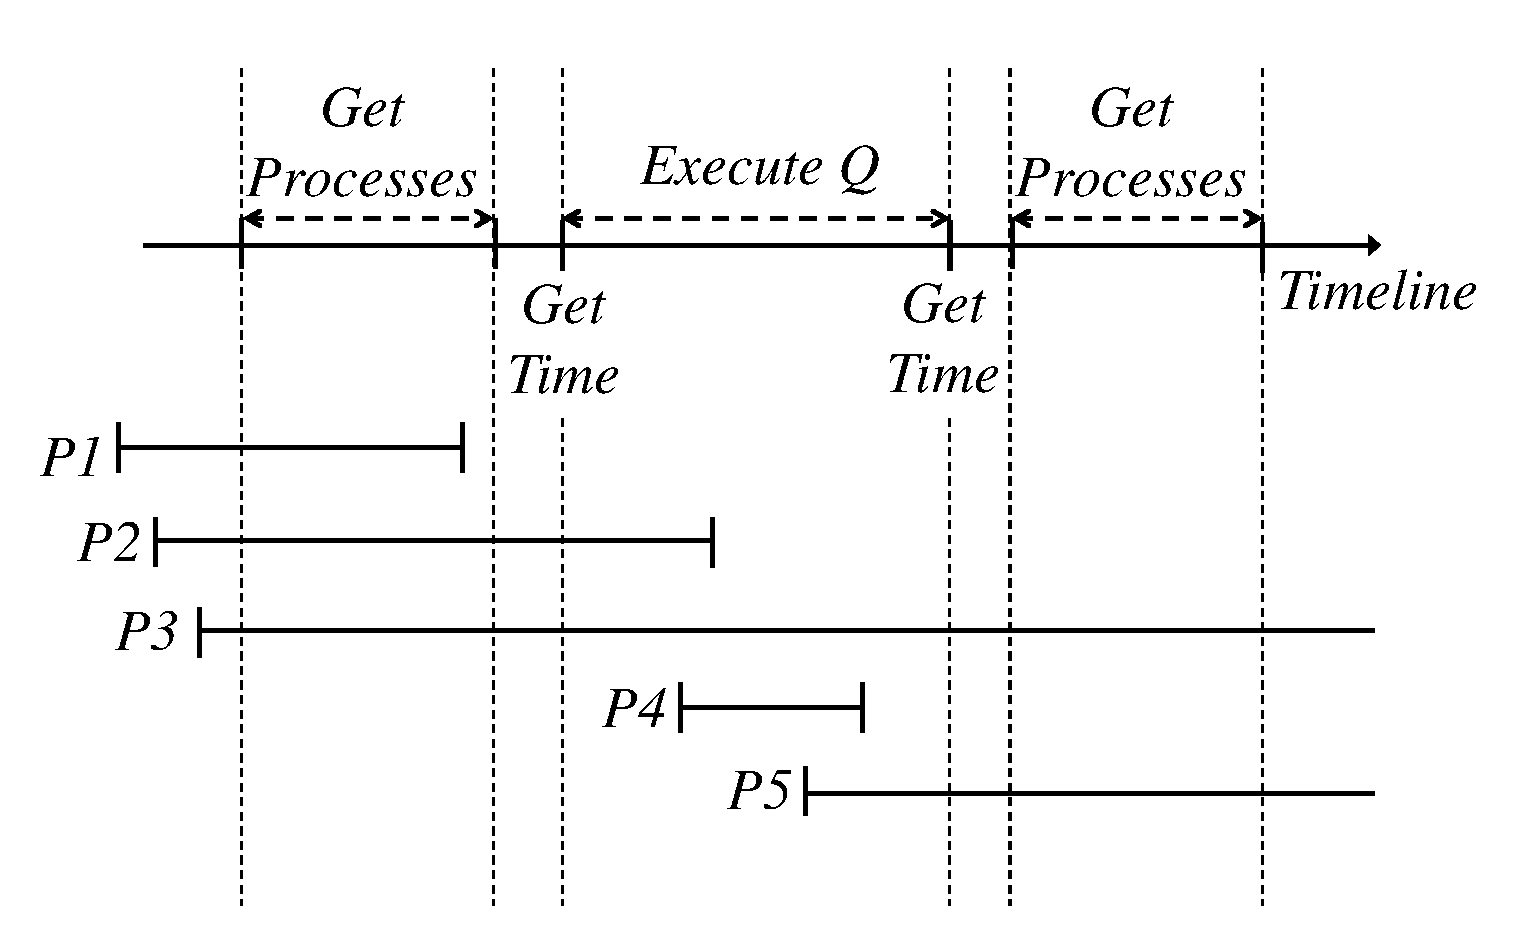
\includegraphics[width=0.50\textwidth]{figures/time_measurement.eps}
\caption{Processes influencing query execution\label{fig:timing}}
\end{figure}

In this section we discuss how we measure query execution time. 
As illustrated in Figure~\ref{fig:timing}, 
we first get all running processes before executing 
a query $Q$. 
Then timer for $Q$ gets started, and it is stopped after $Q$ gets 
executed. 
The execution time for $Q$ is measured by the time difference, and 
we finally finish single query execution by examining running 
processes right after the execution. 

Now let us examine how other processes may influence query execution. 
Assume that all the processes below are not relevant to DBMS processes.
Before timing $Q$, processes $P$1, $P$2 and $P$3 are recorded into 
a map $M$1. 
Another map $M$2, on the contrary, keeps processes $P$3 and $P$5 
captured after the timing. 
For each recorded process, the maps $M$1 and $M$2 keep 
$<$process id (pid), \{process name, minimum/major faults, 
cpu/system times\}$>$. 
The cpu and system times are considered for the subtraction. 
The process information can be achieved by iterating 
{\tt /proc/\{pid\}/stat} associated with each process. 

By comparing $M$1 and $M$2, we easily know that $P$3 and $P$5 affected 
$Q$'s execution; thus, the time spent on $P$3 and $P$5 are subtracted from 
the measured query execution time. 
$P$1 and $P$2 that do not appear in $M$2 must have stopped 
before or during the query execution, respectively. 
We cannot determine whether the query execution is affected by 
these stopped processes. 
For instance, $P$2 is explicitly involved with the execution whereas 
$P$1 not. 
What we can know is that regarding the execution, there were stopped 
processes, such as $P$1 and $P$2, as a result of comparison with 
$M$1 and $M$2. 
This execution, therefore, will be thrown out due to the stopped ones. 

Note that $P$4 is a {\em phantom} process, since it does appear 
in neither $M$1 nor $M$2. 
The existence of phantom process can be known by comparing 
the number of processes from {\tt /proc/stat} before and after execution.
Like stopped processes, we throw out any execution with a phantom process, 
considering measurement accuracy.

\begin{figure}[t]
\begin{center}
\begin{algorithmic}
{\bf Algorithm} timeSingleQueryExecution($i$, $q$, \\
						\hspace{44.0mm}$exPlan$, $card$):
\STATE $plan$ $\leftarrow$ get(Prepared)QueryPlan($q$)
\IF{$plan$ $\neq$ $exPlan$}
	\STATE Error: two different plans are observed \\ 
	at the same cardinality. \\
\ENDIF
\STATE Flush disk drive/OS/DBMS caches. \\
\STATE $M1$ $\leftarrow$ $extractAllRunningProcs$() \\
\STATE $startTime$ $\leftarrow$ $getCurrTimeMills$() \\
\STATE $executeQuery$($q$) \\ 
\STATE $endTime$ $\leftarrow$ $getCurrTimeMills$() \\	
\STATE $execTime$ $\leftarrow$ $endTime$ - $startTime$ \\	
\STATE $M2$ $\leftarrow$ $extractAllRunningProcs$() \\
\STATE $procDiff$ $\leftarrow$ $diff$($M1$, $M2$) \\	
\STATE RecordQueryExecution($i$, $q$, $card$, \\ 
			\hspace{34.0mm}$execTime$, $procDiff$) \\
\end{algorithmic}
\caption{Timing single query excution\label{alg:timing}}
\end{center}
\end{figure}

